\documentclass[12pt,a4paper]{book}
\usepackage{lmodern}
\usepackage{amssymb,amsmath}
\usepackage{ifxetex,ifluatex}
\usepackage{fixltx2e} % provides \textsubscript
\ifnum 0\ifxetex 1\fi\ifluatex 1\fi=0 % if pdftex
  \usepackage[T1]{fontenc}
  \usepackage[utf8]{inputenc}
\else % if luatex or xelatex
  \ifxetex
    \usepackage{mathspec}
  \else
    \usepackage{fontspec}
  \fi
  \defaultfontfeatures{Ligatures=TeX,Scale=MatchLowercase}
\fi
% use upquote if available, for straight quotes in verbatim environments
\IfFileExists{upquote.sty}{\usepackage{upquote}}{}
% use microtype if available
\IfFileExists{microtype.sty}{%
\usepackage{microtype}
\UseMicrotypeSet[protrusion]{basicmath} % disable protrusion for tt fonts
}{}
\usepackage[margin=2cm]{geometry}
\usepackage{hyperref}
\PassOptionsToPackage{usenames,dvipsnames}{color} % color is loaded by hyperref
\hypersetup{unicode=true,
            pdftitle={Notes on a design of a simple spatial sampling method (S3M) for assessing coverage of health and nutrition programmes in Liberia},
            pdfauthor={Valid International},
            colorlinks=true,
            linkcolor=Maroon,
            citecolor=Blue,
            urlcolor=Blue,
            breaklinks=true}
\urlstyle{same}  % don't use monospace font for urls
\usepackage{natbib}
\bibliographystyle{apalike}
\usepackage{longtable,booktabs}
\usepackage{graphicx,grffile}
\makeatletter
\def\maxwidth{\ifdim\Gin@nat@width>\linewidth\linewidth\else\Gin@nat@width\fi}
\def\maxheight{\ifdim\Gin@nat@height>\textheight\textheight\else\Gin@nat@height\fi}
\makeatother
% Scale images if necessary, so that they will not overflow the page
% margins by default, and it is still possible to overwrite the defaults
% using explicit options in \includegraphics[width, height, ...]{}
\setkeys{Gin}{width=\maxwidth,height=\maxheight,keepaspectratio}
\IfFileExists{parskip.sty}{%
\usepackage{parskip}
}{% else
\setlength{\parindent}{0pt}
\setlength{\parskip}{6pt plus 2pt minus 1pt}
}
\setlength{\emergencystretch}{3em}  % prevent overfull lines
\providecommand{\tightlist}{%
  \setlength{\itemsep}{0pt}\setlength{\parskip}{0pt}}
\setcounter{secnumdepth}{5}
% Redefines (sub)paragraphs to behave more like sections
\ifx\paragraph\undefined\else
\let\oldparagraph\paragraph
\renewcommand{\paragraph}[1]{\oldparagraph{#1}\mbox{}}
\fi
\ifx\subparagraph\undefined\else
\let\oldsubparagraph\subparagraph
\renewcommand{\subparagraph}[1]{\oldsubparagraph{#1}\mbox{}}
\fi

%%% Use protect on footnotes to avoid problems with footnotes in titles
\let\rmarkdownfootnote\footnote%
\def\footnote{\protect\rmarkdownfootnote}

%%% Change title format to be more compact
\usepackage{titling}

% Create subtitle command for use in maketitle
\newcommand{\subtitle}[1]{
  \posttitle{
    \begin{center}\large#1\end{center}
    }
}

\setlength{\droptitle}{-2em}
  \title{Notes on a design of a simple spatial sampling method (S3M) for
assessing coverage of health and nutrition programmes in Liberia}
  \pretitle{\vspace{\droptitle}\centering\huge}
  \posttitle{\par}
  \author{Valid International}
  \preauthor{\centering\large\emph}
  \postauthor{\par}
  \predate{\centering\large\emph}
  \postdate{\par}
  \date{2018-06-20}

\usepackage{booktabs}
\usepackage{color}
\usepackage{tcolorbox}
\usepackage{float}
\usepackage{setspace}

\onehalfspacing

\graphicspath{ {icons/} }

\newenvironment{rmdremind}
  {\begin{tcolorbox}[width=\textwidth, 
                     colback = {white}, 
                     title = {\textbf{Remember}}, 
                     colbacktitle = lightgray,
                     coltitle = black]
  \begin{includegraphics}[scale = 1]{remind.png}
  \begin{itemize}}
  {\end{itemize}
  \end{includegraphics}
  \end{tcolorbox}}

\newenvironment{rmdnote}
  {\begin{tcolorbox}[width=\textwidth, 
                     colback = {white}, 
                     title = {\textbf{Note}}, 
                     colbacktitle = lightgray,
                     coltitle = black]
  \begin{includegraphics}[scale = 1]{pencil.png}}
  {\end{includegraphics}
  \end{tcolorbox}}
  
\newenvironment{rmdexercise}
  {\begin{tcolorbox}[width=\textwidth, 
                     colback = {white}, 
                     title = {\textbf{Exercise}}, 
                     colbacktitle = lightgray,
                     coltitle = black]
  \begin{includegraphics}[scale = 1]{exercise.png}}
  {\end{includegraphics}
  \end{tcolorbox}}
  
\newenvironment{rmdbox}
  {\begin{tcolorbox}[width=\textwidth, 
                     colback = {white}, 
                     title = {\textbf{Exercise}}, 
                     colbacktitle = lightgray,
                     coltitle = black]
  \begin{includegraphics}[scale = 1]{pencil.png}}
  {\end{includegraphics}
  \end{tcolorbox}}
  
\newenvironment{rmdinfo}
  {\begin{tcolorbox}[width=\textwidth, 
                     colback = {white}, 
                     title = {\textbf{Info}}, 
                     colbacktitle = lightgray,
                     coltitle = black]
  \begin{includegraphics}[scale = 1]{info.png}}
  {\end{includegraphics}
  \end{tcolorbox}}  
  
\newenvironment{rmdwarning}
  {\begin{tcolorbox}[width=\textwidth, 
                     colback = {white}, 
                     title = {\textbf{Warning}}, 
                     colbacktitle = lightgray,
                     coltitle = black]
  \begin{includegraphics}[scale = 1]{warning.png}}
  {\end{includegraphics}
  \end{tcolorbox}}

\newenvironment{rmddownload}
  {\begin{tcolorbox}[width=\textwidth, 
                     colback = {white}, 
                     title = {\textbf{Download}}, 
                     colbacktitle = lightgray,
                     coltitle = black]
  \begin{includegraphics}[scale = 1]{download.png}}
  {\end{includegraphics}
  \end{tcolorbox}}

\usepackage{amsthm}
\newtheorem{theorem}{Theorem}[chapter]
\newtheorem{lemma}{Lemma}[chapter]
\theoremstyle{definition}
\newtheorem{definition}{Definition}[chapter]
\newtheorem{corollary}{Corollary}[chapter]
\newtheorem{proposition}{Proposition}[chapter]
\theoremstyle{definition}
\newtheorem{example}{Example}[chapter]
\theoremstyle{definition}
\newtheorem{exercise}{Exercise}[chapter]
\theoremstyle{remark}
\newtheorem*{remark}{Remark}
\newtheorem*{solution}{Solution}
\begin{document}
\maketitle

{
\hypersetup{linkcolor=black}
\setcounter{tocdepth}{1}
\tableofcontents
}
\begin{verbatim}
## Warning in rgdal::readOGR(dsn = "maps/lbr_rdsl_unmil", layer =
## "lbr_rdsl_unmil", : Dropping null geometries: 70, 89, 1125, 1253, 2054,
## 2678, 2708, 3190, 3261
\end{verbatim}

\hypertarget{simple-spatial-sampling-method-s3m}{%
\chapter*{Simple Spatial Sampling Method
(S3M)}\label{simple-spatial-sampling-method-s3m}}
\addcontentsline{toc}{chapter}{Simple Spatial Sampling Method (S3M)}

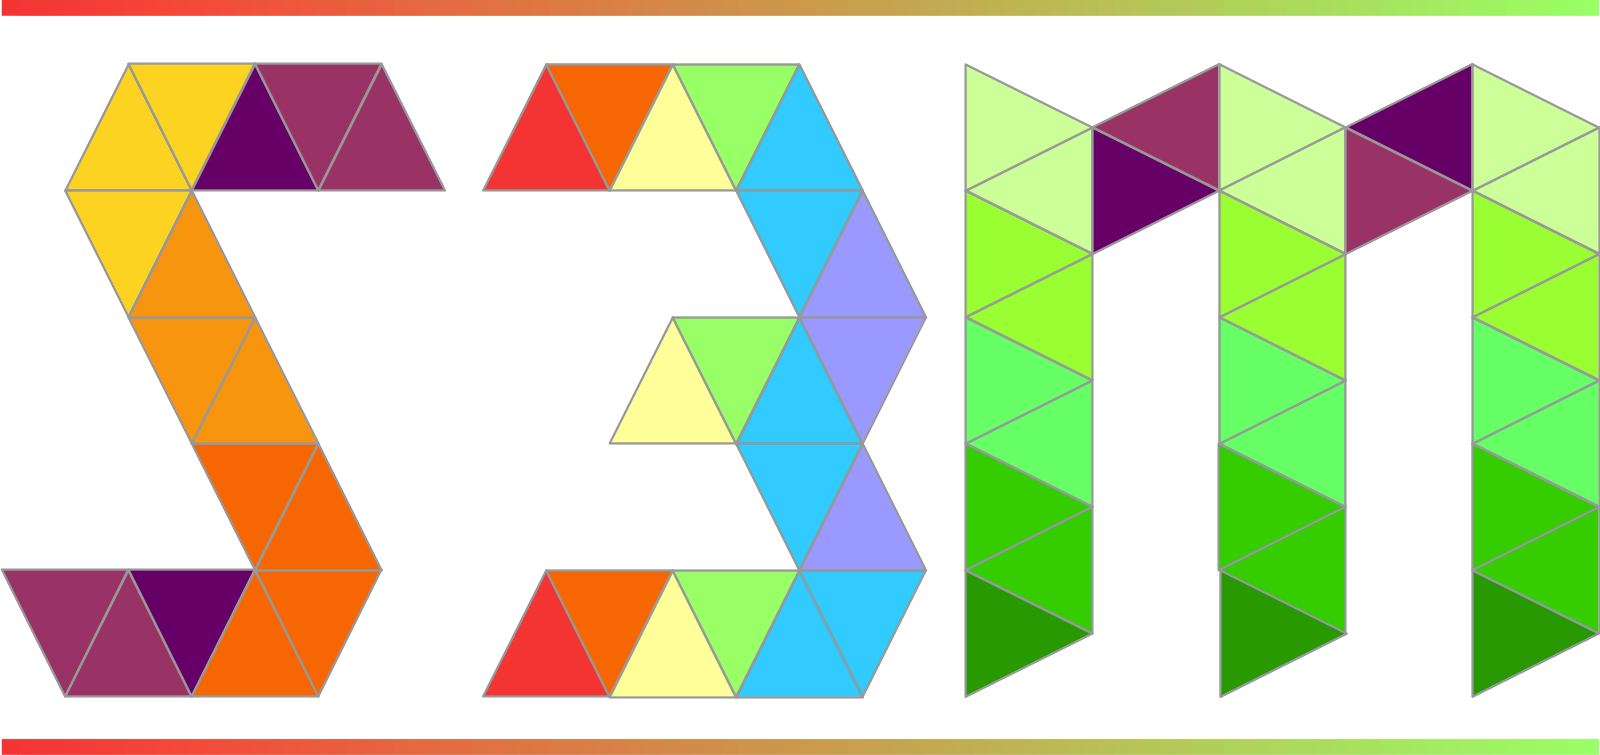
\includegraphics{figures/s3mlogo.png}

\hypertarget{introduction}{%
\chapter{Introduction}\label{introduction}}

The Simple Spatial Survey Method (S3M) was developed from the CSAS
coverage survey method as a response to the widespread adoption of
community management of acute malnutrition (CMAM) by ministries of
health. Large-scale programs need a large-scale survey method and S3M
was developed to meet that need.

S3M was designed to :

\begin{itemize}
\item
  Be simple enough for MoH, NGO, and UNO personnel without specialist
  statistical training to perform.
\item
  Provide a general survey method. S3M can be used to survey and map :
\item
  Need for and coverage of selective-entry programs such as CMAM and
  TSFP as well as universal programs such as EPI, GMP, GFD (general
  ration), and ``blanket'' SFP over wide areas.
\item
  Levels of indicators such as those for IYCF, WASH, and period
  prevalence / cumulative prevalence of ARI, fever, and diarrhoea over
  wide areas.
\end{itemize}

This document concentrates on using S3M to assess the need for and
coverage of a variety of selective-entry feeding programs. The
indicators discussed in this manual are:

\begin{itemize}
\item
  Therapeutic feeding (OTP and TSFP) programs :
\item
  Prevalence of SAM and coverage of treatment of SAM in children aged
  between 6 and 59 months.
\item
  Prevalence of MAM and coverage of treatment of MAM in children aged
  between 6 and 59 months.
\item
  Prevalence of MAM and treatment of MAM and in pregnant and lactating
  women (PLWs).
\item
  Food-based prevention of malnutrition (FBPM) programs :
\item
  Prevalence of need for and coverage of food-based prevention of
  malnutrition in younger children at risk of developing MAM and SAM.
\item
  Prevalence of need for and coverage of food-based prevention of
  malnutrition in pregnant and lactating women (PLWs) at risk of
  developing MAM and SAM.
\item
  Coverage of screening for all of the above programs.
\item
  Coverage of Behaviour Change Communication (BCC) programs focussing on
  maternal and child health and nutrition to all principal carers of
  children (usually their mothers) and all PLWs.
\end{itemize}

\hypertarget{sample}{%
\chapter{The survey sample}\label{sample}}

The survey method described here uses a two-stage sample:

\begin{itemize}
\item
  \textbf{First-stage:} We take an even (or near-even) spatial sample of
  communities from all of the communities in the survey area.
\item
  \textbf{Second-stage:} We take a sample of eligible individuals from
  each of the communities identified in the first stage of sampling.
\end{itemize}

Two-stage sampling is used in many survey methods. A typical example of
a survey method that uses a two- stage sample is the SMART method that
is commonly used for nutritional anthropometry surveys.

The main difference between the sample taken in S3M based surveys and in
SMART type surveys is that S3M based samples used a spatial sample in
the first stage whereas SMART type surveys use a proportional to
population size (PPS) sample.

The advantages of using a spatial first stage sample is that such a
sample allows us to identify where (and why) coverage is good, and where
(and why) coverage is poor. This information is essential to improving
program coverage and ensuring equitable access to services.

A spatial sample can be used to produce equivalent results to a
traditional proportional to population size (PPS) sample as is used in
(e.g.) SMART type surveys using a weighted analysis. This means that a
spatial sample can be made to act as a PPS sample. A PPS type sample
cannot, however, be made to act as a spatial sample.

\hypertarget{stage1}{%
\chapter{The first stage sample}\label{stage1}}

\hypertarget{step-1-find-a-map}{%
\section{Step 1: Find a map}\label{step-1-find-a-map}}

The first step in a S3M survey is to find a map of the survey area. A
map showing the locations of all towns and villages in the survey area
is essential. Try to find a map showing the locations of all towns and
villages in the survey area. You may need to update the map to take into
account migration and displacement.

For the coverage survey of 2 counties in Liberia, it will be practical
and useful to have:

\begin{itemize}
\tightlist
\item
  A small scale-map (a wide area map but with poor detail) of the entire
  survey area for each of the 2 counties. If the counties are contiguous
  (i.e., share borders with each other), the small scale map can be of
  the two counties together. This map does not need to show the location
  of all towns and villages in the survey area but it gives a general
  idea of where the 2 counties are located and main towns and location
  and roads.
\end{itemize}

\newpage

\begin{figure}[H]

{\centering 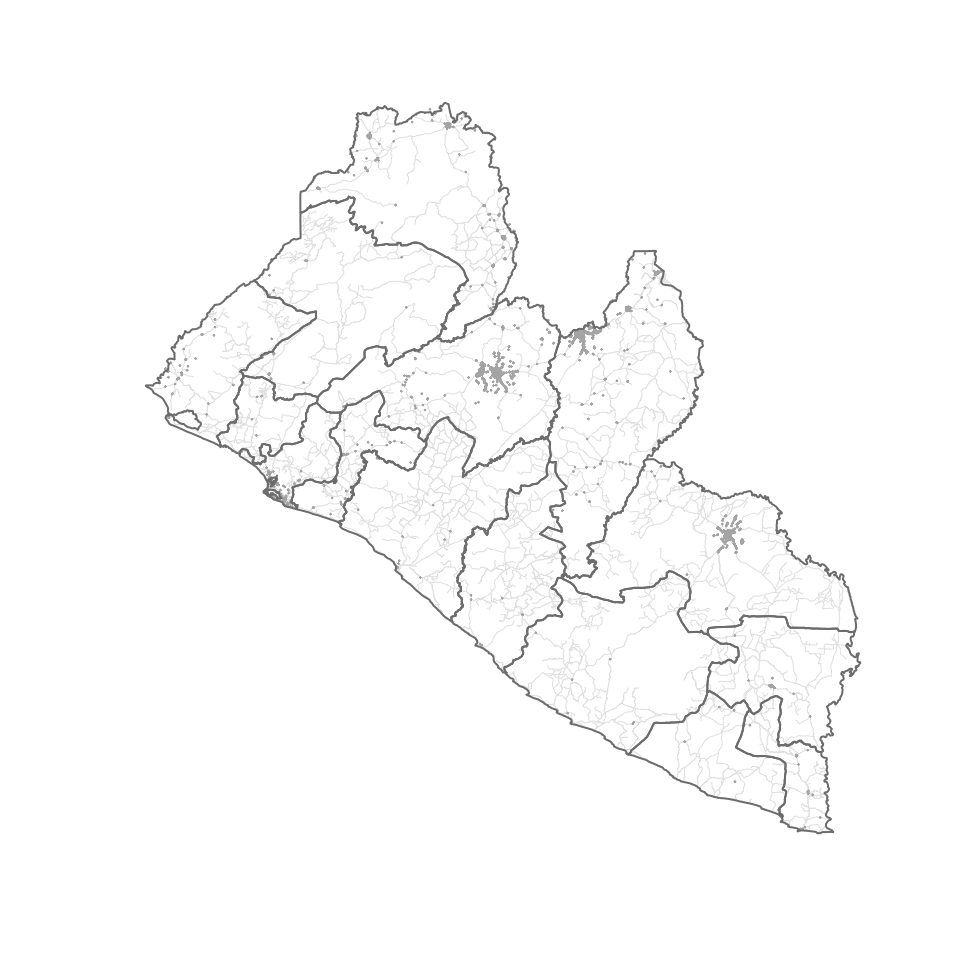
\includegraphics{figures/smallScaleMap-1} 

}

\caption{Small scale map of Liberia showing counties, roads and points of interest}\label{fig:smallScaleMap}
\end{figure}

\newpage

A collection of larger scale maps (a small area map but with good
detail) of each of the five regions of Niger showing the locations of
all towns and villages. A large-scale map of Dosso found in Figure 2 is
a good example. The Humanitarian Information Centre (HIC) in Niamey is a
good resource for obtaining these maps. The small-scale map in Figure 1
will be useful for identifying initial sampling locations. The large-
scale maps will be useful for identifying the precise location of
sampling points and for selecting the communities to be sampled.

The first step in an S3M survey is to find a map of the survey area.

Try to find a map showing the locations of all towns and villages in the
survey area. You may need to update the map to take into account
migration and displacement.

If you are surveying a very large area then you will find it useful to
have:

\begin{itemize}
\item
  A small scale map of the entire survey area. This map does not need to
  show the location of all towns and villages in survey area.
\item
  A collection of larger scale maps showing the locations of all towns
  and villages. This collection of maps should cover the entire survey
  area.
\end{itemize}

The small scale map will be useful for identifying initial sampling
locations.

The large scale maps will be useful for identifying the precise
locations of sampling points and for selecting the communities to be
sampled.

\hypertarget{stage2}{%
\chapter{The second stage sample}\label{stage2}}

\hypertarget{analysis}{%
\chapter{Analysis}\label{analysis}}

\bibliography{book.bib}


\end{document}
